% LAB 9: Matplotlib
%
% CSE/IT 107: Introduction to Programming
% New Mexico Tech
%
% Prepared by Stephanie Gott and Hugo Rivera
% Spring 2016
\documentclass[11pt]{cselabheader}
\usepackage{float}

%%%%%%%%%%%%%%%%%% SET TITLES %%%%%%%%%%%%%%%%%%%%%%%%%
\fancyhead[R]{Lab 9: Matplotlib}
\title{Lab 9: Matplotlib}

\begin{document}

\maketitle
\pagenumbering{roman}
\hrule

\begin{quote}
``The greatest value of a picture is when it forces us to notice what we
never expected to see.''
\end{quote}
\begin{flushright}
---John Tukey
\end{flushright}

\begin{figure}[H]
  \centering
  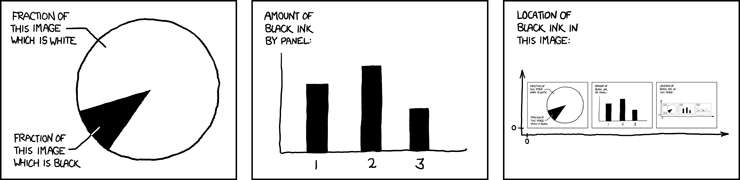
\includegraphics[width=\textwidth]{img/xkcd_self_description.png}
  \caption{Self description. \url{https://xkcd.com/688/}}
\end{figure}

\hrule

\pagebreak
\tableofcontents

\section*{Introduction}
\addcontentsline{toc}{section}{Introduction}
In this lab you will learn about generating 2D graphics using
Matplotlib.  This is a powerful Python library that can be used to
create detailed visualizations such as scatter plots and
histograms. You will learn to about Python's list comprehensions,
which help when modifying lists of data.  There's also an extra credit
where you use the CSV module to read CSV files.  The key lesson of
this lab is learning to read Python library documentation. With this
skill you can learn to use many of Python's free and open-source
libraries.

\pagebreak
\pagenumbering{arabic}
\section{Keyword Arguments}
Before we start, you should know about a commonly used Python feature
called keyword arguments. As you know, functions may take zero or more
required arguments, these are called \textsl{positional arguments}.
There is a special syntax that can be used to define \textsl{optional
arguments.}

For example, this function takes either one or two arguments. The second
argument has a default value of 5.

\begin{pyconcode}
>>> def f(fst, snd = 5):
...    return fst * snd
>>> f(10)
50
>>> f(10, 6)
60
>>> f()
Traceback (most recent call last):
  File ``<stdin>'', line 1, in <module>
TypeError: f() missing 1 required positional argument: 'fst'
\end{pyconcode}

An important feature is that keyword arguments may be labeled
and listed in any order when calling the function. For example,
the following function takes two keyword arguments. There are five
valid ways to call this function.

\begin{pyconcode}
>>> def p(greeting="Hello", subject="world"):
...     return "{} {}".format(greeting, subject)
>>> p()
"Hello world"
>>> p(greeting="Goodbye")
"Goodbye world"
>>> p(subject="humans")
"Hello humans"
>>> p(greeting="Bonjour", subject="le monde")
"Bonjour le monde"
>>> p(subject="le monde", greeting="Bonjour")
"Bonjour le monde"
\end{pyconcode}

% \section{Numpy Arrays}
% Before we can use Matplotlib, we must learn about a new datatype:
% Numpy arrays.  These are efficient containers for numeric data and
% prefered when plotting data using Matplotlib. There are several ways
% to construct these arrays. The \pythoninline{numpy.array()} function
% can be used to convert a Python list into an array.
%
%   \begin{pyconcode}
% >>> import numpy
% >>> xs = numpy.array([1,2,3])
% array([1, 2, 3])
% >>> ys = numpy.array([8,4,7])
% array([8, 4, 7])
%   \end{pyconcode}
%
% The \pythoninline{numpy.linspace} can be used to create evenly spaced values.
% For example, if we want 10 points between 0 and 1 (inclusive), we can type:
%   \begin{pyconcode}
% >>> import numpy
% >>> numpy.linspace(0, 10, num=5)
% array([0, 2.5, 5, 7.5, 10])
%   \end{pyconcode}
%
% You can add or multiply two arrays element-by-element, and you can
% apply other mathematical functions to arrays. For example, the
% \pythoninline{numpy.sqrt} function can be used to find the square root
% of each element in the array.
%   \begin{pyconcode}
% >>> import numpy
% >>> xs = numpy.linspace(0, 1, num=5)
% array([0, 2.5, 5, 7.5, 10])
% >>> os = numpy.linspace(-20, 0, num=5)
% array([-20, -15, -10, -5, 0])
% >>> xs + os
% array([-20, -12.5, -5, 2.5, 10])
% >>> xs * os
% array([0, -37.5, -50, -37.5, 0])
% >>> numpy.sqrt(xs)
% array([0, 1.58113883, 2.23606798, 2.73861279, 3.16227766])
% >>> numpy.sin(os)
% array([-0.91294525, -0.65028784, 0.54402111, 0.95892427, 0])
%   \end{pyconcode}
%
% The \pythoninline{numpy.arange} function is similar to Python's
% \pythoninline{range} function. It improves on the built-function by
% generating values spaced by non-integers.
%
% \begin{pyconcode}
% >>> import numpy
% >>> numpy.arange(0, 10)
% array([0, 1, 2, 3, 4, 5, 6, 7, 8, 9])
% >>> numpy.arange(0, 12, 3)
% array([0, 3, 6, 9])
% >>> numpy.arange(0, 4, 0.5)
% array([0.0, 0.5, 1.0, 1.5, 2.0, 2.5, 3.0, 3.5])
% \end{pyconcode}

\section{List Comprehensions}
\subsection{Modifying Collections}

List comprehensions can be used to modify lists by doing something to
each element.  For example, if we want to make every string in a list
of strings lowercase we can use a for-loop call \pythoninline{.lower()}
on each string.

\begin{pyconcode}
>>> strings = ["Python", "N.M."]
>>> result = []
>>> for string in strings:
...    result.append(string.lower())
... print(result)
["python", "n.m."]
\end{pyconcode}

List comprehensions are a more concise way of doing this.

\begin{pyconcode}
>>> result = [string.lower() for string in strings]
>>> print(result)
["python", "n.m."]
\end{pyconcode}

We can process more complicated elements with list comprehensions.
If we have a list of dictionaries containing lists, we can find the maximum
element in each sublist by using this list comprehension:

\begin{pyconcode}
>>> data = [{'d': [1,2,3]},
...         {'d': [0,0,1]}]
>>> [max(dictionary['d']) for dictionary in data]
[3, 1]
\end{pyconcode}

\subsection{Filtering Elements}

What if we want to exclude elements? In this code, we take a list of words
and keep all words of length less than 2.

\begin{pyconcode}
>>> strings = ['a', 'ab', 'abb', 'aab']
>>> result = []
>>> for string in strings:
...    if len(string) <= 2:
...        result.append(string)
... print(result)
['a', 'ab']
\end{pyconcode}

This can be written more concisely by using an \pythoninline{if}
statement within a list comprehension.

\begin{pyconcode}
>>> strings = ['a', 'ab', 'abb', 'aab']
>>> [x for x in strings if len(x) <= 2]
['a', 'ab']
\end{pyconcode}

\subsection{Nested Comprehensions}

We can also write multiple \pythoninline{for} statements and
\pythoninline{if} statements in a list comprehension.
This example creates a list of floating point numbers by dividing
two integers

\begin{pyconcode}
>>> result = [y / x for x in range(10) if x != 0 for y in range(10)]
>>> print(result)
[0.0, 1.0, 2.0, 3.0, 4.0, 5.0, 6.0, 7.0, 8.0, 9.0, 0.0, 0.5, 1.0, 1.5,
2.0, 2.5, 3.0, 3.5, 4.0, 4.5, 0.0, 0.3333333333333333, 0.6666666666666666, ...
\end{pyconcode}

These statements should be read from right to left. So the previous list
comprehension is the same as these nested statements:

\begin{python3code}
result = []
for x in range(10):
    if x != 0:
        for y in range(10):
            result.append(y / x)
\end{python3code}

\section{Matplotlib}

Matplotlib is a Python 2D plotting library which produces publication
quality figures in a variety of formats and interactive environments.
We will be using the \pythoninline{matplotlib.pyplot} library. It is
commonly renamed to \pythoninline{plt} using this code:

\begin{pyconcode}
>>> import matplotlib.pyplot as plt
\end{pyconcode}

It's a good idea to keep the Matplotlib documentation on hand as you read these
examples. All of the following matplotlib functions are documented online at:
\begin{center}
\url{http://matplotlib.org/api/pyplot_api.html}
\end{center}

\subsection{Plotting Points with the \protect{\pythoninline{plot}} Function}

\pythoninline{plt.plot} is a versatile function that is used to plot
pairs of numeric values. Matplotlib does not take a list of tuples
representing points, instead it takes two lists. The list of values on
the x-axis are the first argument and the list of y-axis values form
the second argument. One of the lists must be in increasing order.

\begin{pyconcode}
>>> import matplotlib.pyplot as plt
>>> plt.plot([1, 2, 3, 4], [10, -10, 40, 50])
>>> plt.show()
\end{pyconcode}

\begin{center}
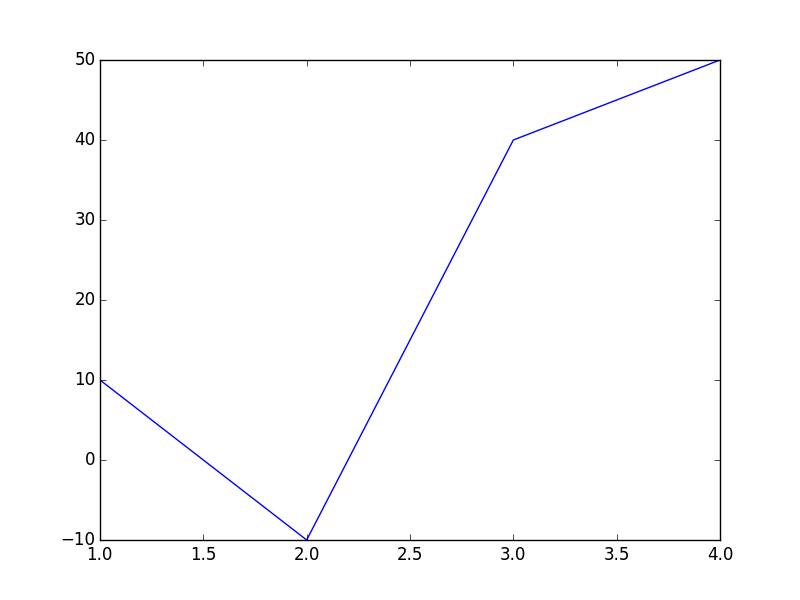
\includegraphics[width=0.6\textwidth]{img/matplotlib_plot1.png}
\end{center}

Note the \pythoninline{plt.show()} function shows everything drawn by
previously called plotting functions.

Matplotlib plots can be modified in many ways. The documentation has a
table of keyword arguments for this function. The columns are Property
and Description.  Let's try some of those. The \pythoninline{color},
\pythoninline{linestyle}, and \pythoninline{marker} keyword arguments
can be used to draw a differently styled line.  As of March, 2016 the
Matplotlib documentation for these functions, colors, and line styles
are located at

\begin{center}
\url{http://matplotlib.org/api/pyplot_api.html#matplotlib.pyplot.plot}

\url{http://matplotlib.org/api/colors_api.html}

\url{http://matplotlib.org/api/lines_api.html#matplotlib.lines.Line2D.set_linestyle}
\end{center}

Here's the same plot with a red, dashed line and o's on every data point.

\begin{pyconcode}
>>> import matplotlib.pyplot as plt
>>> plt.plot([1, 2, 3, 4, 5], [10, -10, 40, 50, 60],
...          color='red', linestyle='dashed', marker='o')
>>> plt.show()
\end{pyconcode}

\begin{center}
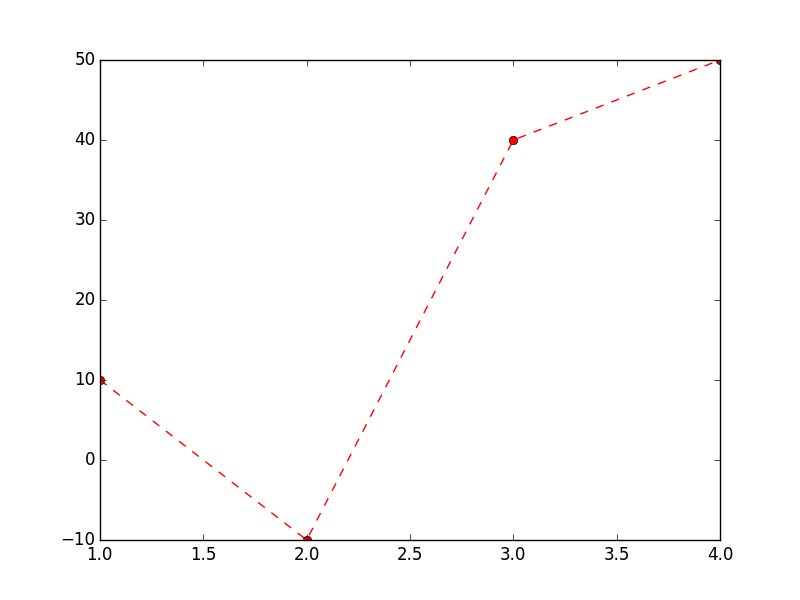
\includegraphics[width=0.6\textwidth]{img/matplotlib_plot2.png}
\end{center}

\subsection{Histograms using the \protect{\pythoninline{hist}}
Function}

Matplotlib's \pythoninline{plt.hist()} can draw the histogram of a
list, which shows how often a value occurs.

\begin{pyconcode}
>>> import matplotlib.pyplot as plt
>>> plt.hist([1, 1, 1, 1.2, 1.3, 1.9, 1.9, 2, 2.1, 2.5])
>>> plt.show()
\end{pyconcode}

\begin{center}
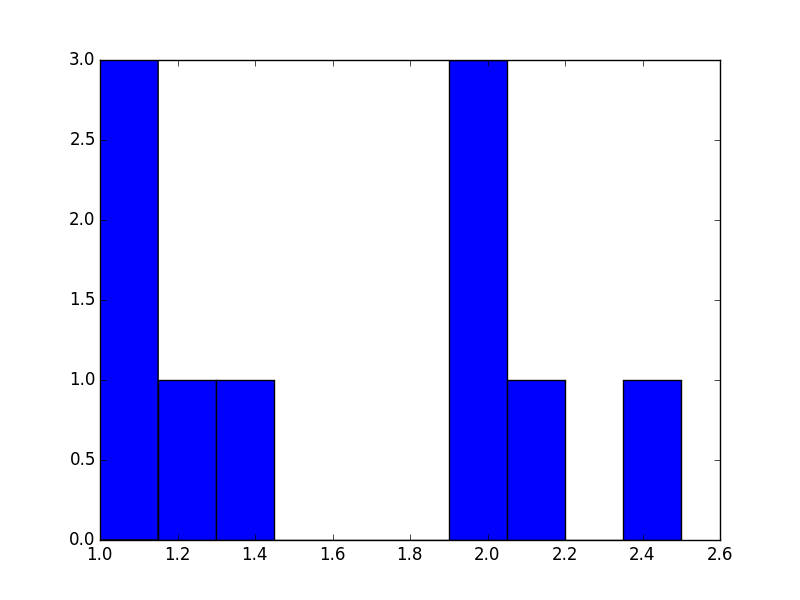
\includegraphics[width=0.6\textwidth]{img/matplotlib_hist1.png}
\end{center}

The \pythoninline{bins} argument is used to draw fewer bins of
data. The histogram is rotated by setting
\pythoninline{orientation='horizontal'}. See the documentation at:

\begin{center}
\url{http://matplotlib.org/api/pyplot_api.html#matplotlib.pyplot.hist}
\end{center}

\begin{pyconcode}
>>> import matplotlib.pyplot as plt
>>> plt.hist([1, 1, 1, 1.2, 1.3, 1.9, 1.9, 2, 2.1, 2.5]),
...          bins=4, orientation='horizontal', color='red')
>>> plt.show()
\end{pyconcode}

\begin{center}
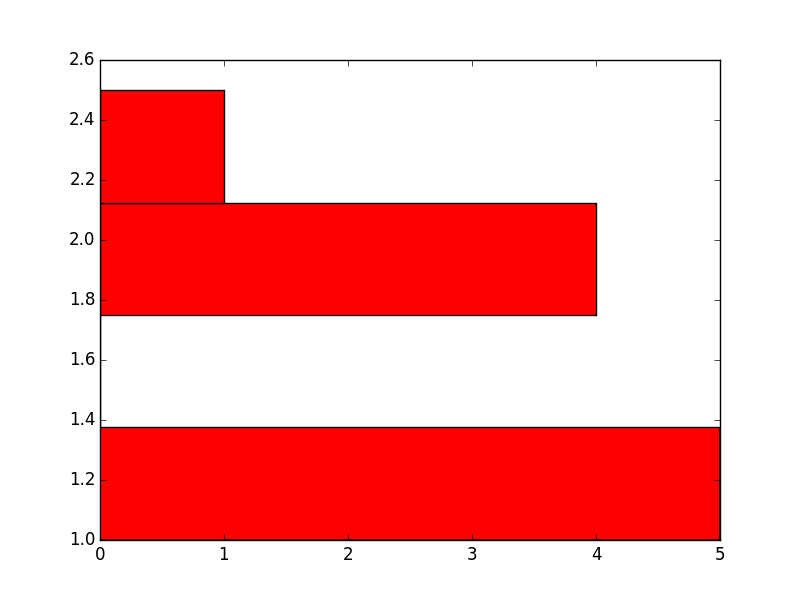
\includegraphics[width=0.6\textwidth]{img/matplotlib_hist2.png}
\end{center}

\subsection{Scatter plots with \protect{\pythoninline{scatter}} Function}

Scatter plots may be generated using the \pythoninline{plt.scatter} function.
These plots should be given three arguments \pythoninline{x, y, s}; these are
arrays indicating the x and y values of the data and the size of each data point.
The \pythoninline{c} and \pythoninline{alpha} keyword arguments can be used to
modify color and opacity of data points. Colors are automatically picked if an
array of values is given. Documentation available at

\begin{center}
\url{http://matplotlib.org/api/pyplot_api.html#matplotlib.pyplot.hist}
\end{center}

This plots data with ordered x-values between 0 and 10, randomly generated
y-values between 0 and 10, and sizes between 1200 and 10 with some variation.
The color scheme are automatically picked according to size.

\begin{pyconcode}
>>> import numpy as np
>>> import matplotlib.pyplot as plt
>>> x = np.linspace(0, 10, num=20)
>>> y = np.random.random(20) * 10
>>> sizes = np.linspace(1200, 30, num=20) + np.random.random() * 100
>>> plt.scatter(x, y, s=sizes, c=sizes, alpha=0.8)
>>> plt.show()
\end{pyconcode}

\begin{center}

\includegraphics[width=0.8\textwidth]{img/matplotlib_scatter.png}
\end{center}

\subsection{Bar Plots with the \protect{\pythoninline{bar}} Function}

Matplotlib can draw a plot of rectangles, each one bounded by the four edges:
\pythoninline{left}, \pythoninline{left + width}, \pythoninline{bottom}, and
\pythoninline{bottom + height}. Here's a demonstration using the
\pythoninline{color} and \pythoninline{edgecolor} keyword arguments.
Documentation is here:

\begin{center}
\url{http://matplotlib.org/api/pyplot_api.html#matplotlib.pyplot.bar}
\end{center}


The rectangles have randomly generated heights and the same width and space
between them.

\begin{pyconcode}
>>> import numpy as np
>>> import matplotlib.pyplot as plt
>>> lefts = np.arange(0, 100, 5)
>>> heights = np.random.random(20) * 50 + 10
>>> plt.bar(left=lefts, height=heights, width=4.5, bottom=0,
...         color='lightblue', edgecolor='blue')
>>> plt.show()
\end{pyconcode}

\begin{center}
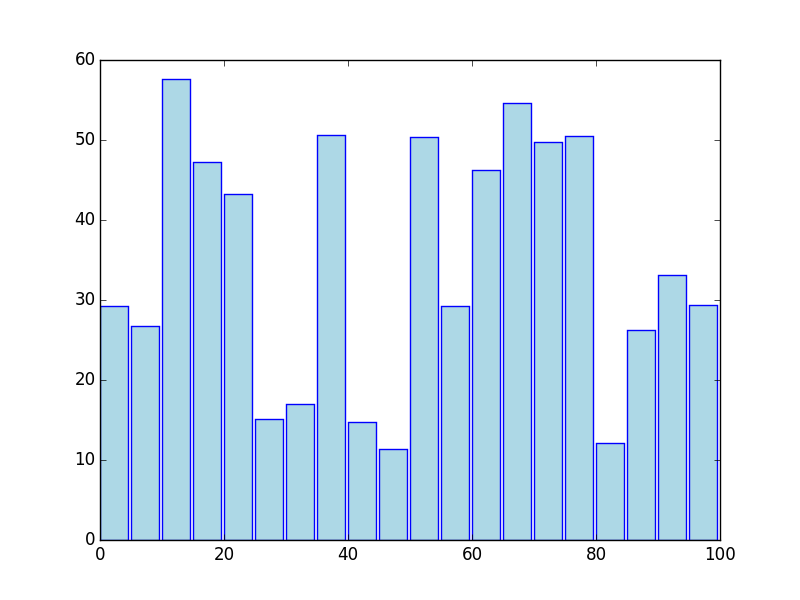
\includegraphics[width=0.6\textwidth]{img/matplotlib_bar.png}
\end{center}

\subsection{Drawing Many Plots with the \protect{\pythoninline{subplot}}
Function}

If you want to draw many plots in the same figure, use the
\pythoninline{plt.subplot} function to split the figure into several rows
and columns. The first and second arguments are the number of rows and columns.
The third argument is the figure number, this should be between 1 and
rows * columns. Documentation available at

\begin{center}
\url{http://matplotlib.org/api/pyplot_api.html#matplotlib.pyplot.subplot}
\end{center}

Here we draw 4 plots, three \pythoninline{plt.plot}s and one
\pythoninline{plt.hist} at the bottom corner.

\begin{python3code}
import numpy as np
import matplotlib.pyplot as plt
x = np.linspace(0, 10, num=20)
y = np.random.random(20)

plt.subplot(2, 2, 1)
plt.plot(x, y)

plt.subplot(2, 2, 2)
plt.plot(x, 0.5 * x ** 2)

plt.subplot(2, 2, 3)
plt.plot(x, y * x ** 2)

plt.subplot(2, 2, 4)
plt.hist(y)

plt.show()
\end{python3code}

\begin{center}
  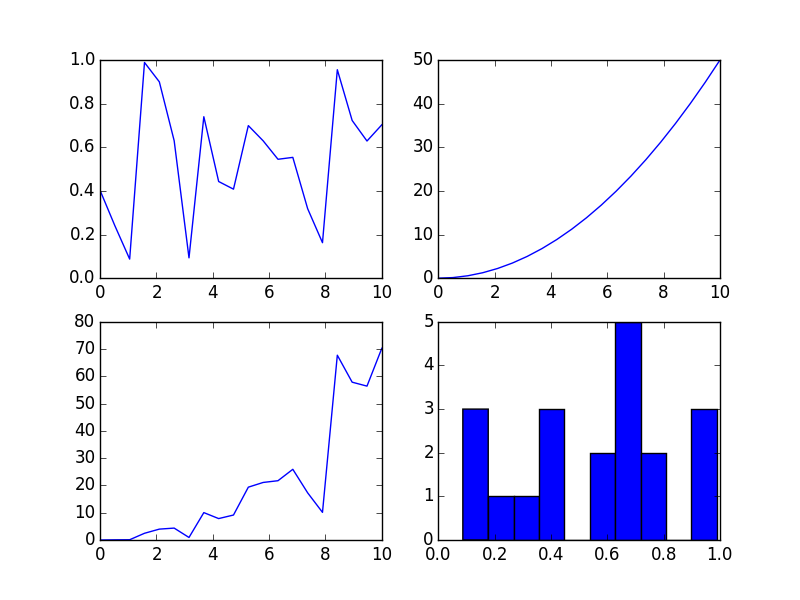
\includegraphics[width=\textwidth]{img/matplotlib_subplot.png}
\end{center}

\subsection{Describing your Plots}
See these links for documentation:
\begin{center}
\url{http://matplotlib.org/api/pyplot_api.html#matplotlib.pyplot.xlabel}

\url{http://matplotlib.org/api/pyplot_api.html#matplotlib.pyplot.ylabel}

\url{http://matplotlib.org/api/pyplot_api.html#matplotlib.pyplot.title}

\url{http://matplotlib.org/api/pyplot_api.html#matplotlib.pyplot.subplot}
\end{center}

Plots can be labeled and titled using the
\pythoninline{plt.xlabel},
\pythoninline{plt.ylabel},
and \pythoninline{plt.title} functions.
Here's an example:

\begin{python3code}
import numpy as np
import matplotlib.pyplot as plt
x = np.linspace(0, 50, num=20)
y = np.random.random(20) * x + x

plt.plot(x, y)
plt.xlabel('Time spent coding')
plt.ylabel('Winning')
plt.title('Data plot.')
plt.show()
\end{python3code}

\begin{center}
  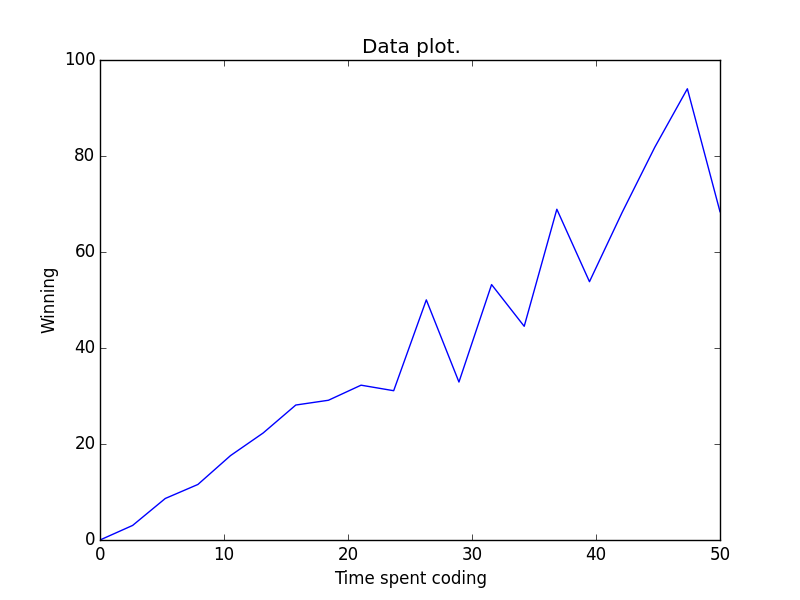
\includegraphics[width=0.6\textwidth]{img/matplotlib_labeled1.png}
\end{center}

What if you want to call attention to an individual data point? Then
you should consider the \pythoninline{plt.annotate} function to add
annotations to plots.  In this example we indicate the maximum y-value
in a randomly generated set of data: This code produces a labeled,
annotated plot.

Annotation text is set with the \pythoninline{s} argument. The arrow
is styled using the \pythoninline{arrowprops} argument.  The
\pythoninline{xy} and \pythoninline{xytext} keyword arguments are used
to place the arrow and text.

\begin{python3code}
import numpy as np
import matplotlib.pyplot as plt
x = np.linspace(0, 50, num=20)
y = np.random.random(20) * x + x

# find maximum
maximum_index = np.argmax(y)
maximum = y[maximum_index]

plt.plot(x, y)
plt.xlabel('Time spent coding')
plt.ylabel('Winning')
plt.title('Data plot.')

# add annotation at maximum point
plt.annotate(s='Maximum value is {:.3}'.format(y[maximum_index]),
             xy=(x[maximum_index], y[maximum_index]),
             xytext=(x[maximum_index] * 0.6, y[maximum_index] * 0.9),
             arrowprops={'arrowstyle': "wedge,tail_width=0.25"})

plt.show()
\end{python3code}

\begin{center}
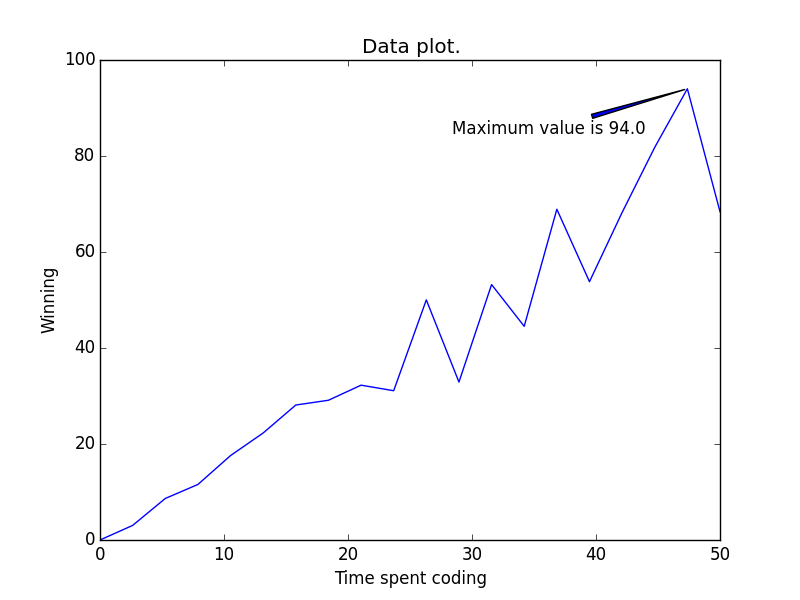
\includegraphics[width=0.6\textwidth]{img/matplotlib_labeled2.png}
\end{center}

\subsection{Subplots and Annotations}

Here's an example where subplots have annotations and titles.

\begin{python3code}
import numpy as np
import matplotlib.pyplot as plt
x = [1, 2, 3, 4, 5]
y1 = [4, 8, 2, 6, 0]
y2 = [14, 2, 8, 0, 1]

plt.subplot(1, 2, 1)
plt.plot(x, y1)
plt.annotate(s='Here is an 8', xy=(2, 8), xytext=(3,7),
             arrowprops={'arrowstyle': "wedge,tail_width=0.25"})
plt.title('Dataset 1')

plt.subplot(1, 2, 2)
plt.plot(x, y2)
plt.annotate(s='Here is another 8', xy=(3, 8), xytext=(2,9),
             arrowprops={'arrowstyle': "wedge,tail_width=0.25"})
plt.title('Dataset 2')

plt.show()
\end{python3code}

\begin{center}
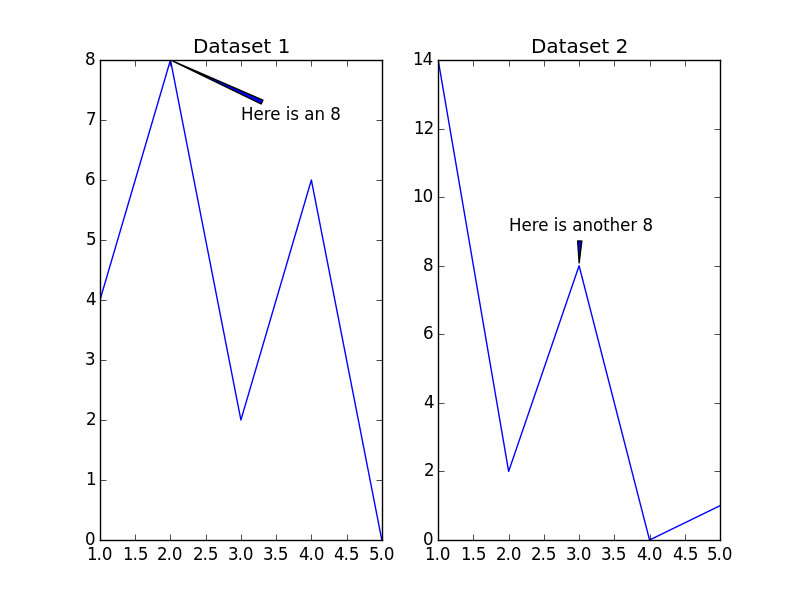
\includegraphics[width=\textwidth]{img/matplotlib_labeledsubplot.png}
\end{center}

\subsection{Overlaying Plots}
Plots may be overlayed by calling plot functions multiple times.
For example, here are plots of two data sets on the same figure.
There is also a line drawn at y=8.

\begin{python3code}
import numpy as np
import matplotlib.pyplot as plt
x = [1, 2, 3, 4, 5]
y1 = [4, 8, 2, 6, 0]
y2 = [14, 2, 8, 0, 1]

plt.plot(x, y1)
plt.plot(x, y2)
plt.plot([1,5], [8,8])
plt.title('Datasets 1 and 2')

plt.show()
\end{python3code}

\begin{center}
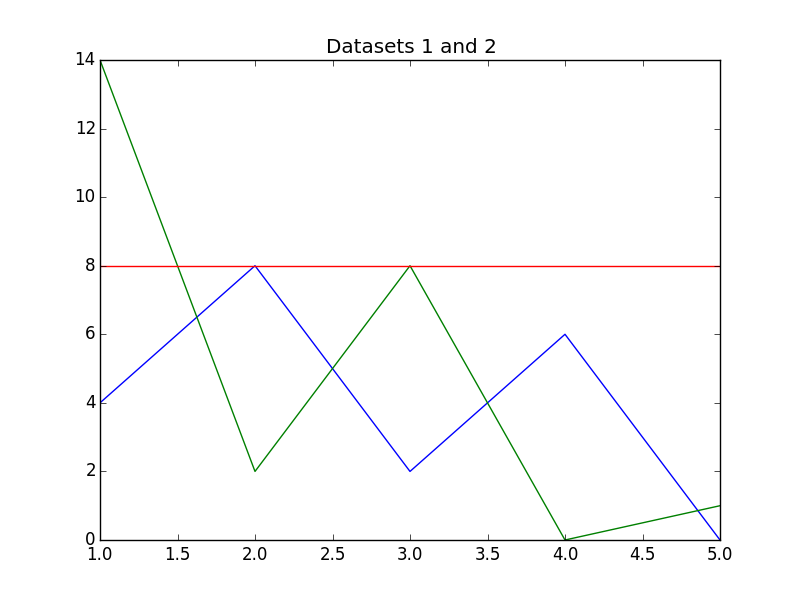
\includegraphics[width=\textwidth]{img/matplotlib_overlayed.png}
\end{center}

\section{Exploring APIs}
An important part of this lab is reading module documentation. You
have already seen two third party modules (Matplotlib and Numpy), and
built-in modules such as \pythoninline{math}. Almost every good Python
module has good documentation and if you want expertise in a module,
you should start reading its documentation.  For example, Matplotlib
supports animation, image rendering, stream plots, error plots,
contour plots, log scaled axis, and many other features. You can see
examples and detailed specifications in the Matplotlib docs.

\subsection{Other Libraries}
Other powerful, third-party and well-documented Python modules include
\begin{inparaenum}
\item \textsl{Scrapy:} a web crawling library.
\item \textsl{Newspaper:} an Easy to use natural language processor and news downloader.
\item \textsl{astropy:} astronomy and astrophysics packages.
\item \textsl{vtk:} highly functional 3D visualization library.
\item \textsl{pillow:} the friendly fork of the Python Imaging Library.
\item \textsl{OpenCV:} a computer vision library.
\item \textsl{Django:} used to deliver and manage dynamic websites; powers many large websites.
\end{inparaenum}

Visit their websites for information on usage and installation.
Here's a list of more interesting libraries:
\begin{center}
\url{https://github.com/vinta/awesome-python}
\end{center}

\newpage
\section{Exercises}
\begin{ex}[plotpoints.py]
Plot the following points. Add labels, a title, and an annotation to the plot
as shown in the example. Make sure to draw a dashed blue line.
The annotation contains the text ``max'' and is located at the point (2, 20).
The annotation text must be slightly below and the arrow connecting the text
and point must be black and have width set to 2.

\begin{python3code}
x = [1,2,3,4,5]
y = [10,20,15,5,-10]
\end{python3code}

\begin{center}
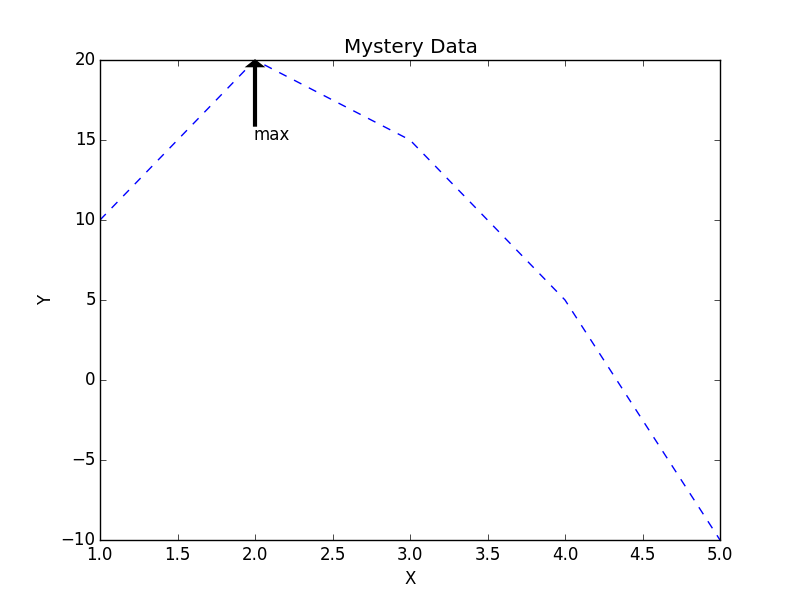
\includegraphics[width=0.5\textwidth]{img/basic.png}
\end{center}
\end{ex}

\begin{ex}[plotscores.py]
  This exercise relies on the \texttt{readscores.py} file from the File I/O
  lab. You may also rewrite that code using the CSV module.

  Write a program that generates the following charts:
  \begin{enumerate}
    \item A histogram of average ACT scores with bins of size $1$ between a
      score of $18$ and $24$.
    \item A bar chart where each state/territory is represented by two
      bars, one for the composite ACT score and the other for the total
      score of all 3 SAT tests.

      Each SAT section is out of 800 points, while the ACT is out of
      36 points.  Use these numbers to modify the data so that both bar
      charts have the same maximum heights.
    \item Produce the same chart as in part 2, but only for states in which
      less than 50\% take the ACT and more than 50\% take the SAT. (There
      should be 21 states/territories like this.)
  \end{enumerate}

  Remember to label your axes and title your graph.
\end{ex}

\begin{infobox}{Supplementary Files}
The \texttt{actsat.txt} file is available on canvas as a lab 7 file.
\end{infobox}

\begin{ex}[plotcountries.py]
Use matplotlib to draw scatter plots relating worldwide life expectancy,
income per person, and population for the years 2010 and 1960.

You may access the data by completing the extra credit or by importing
\texttt{country\_data.py}. The data is stored in the \pythoninline{data1960}
and \pythoninline{2010} values and looks like:

\begin{python3code}
data1960 = [{'country': 'Andorra',
    'expectancy': None,
    'gdp': 15234.0,
    'population': 13414.0},
   {'country': 'Eritrea',
    'expectancy': 41.8278,
    'gdp': 885.0,
    'population': 1407631.0}, ...
\end{python3code}

Notice the special value \pythoninline{None} is present.
To check if a variable \pythoninline{x} is \pythoninline{None},
type \pythoninline{x == None} or \pythoninline{x is None}.


You are required to:

\begin{enumerate}
\item Draw a scatter plot with x and y coordinates set to income and life
expectancy. If there is a \pythoninline{None} value, replace it with the
minimum income or the minimum life expectancy.

\item The area of each data point should be related to the population of every
country. You can choose how to scale the data, but to make it look like the
example, you may use:

\begin{python3code}
scaled_pop = [800 * p / max(pop) for p in pop]
\end{python3code}

\item The scatter plots must be labeled and titled. X label: ``Income'', y
label: ``Life expectancy'', title: ``Year (year of data)''.

\item Annotate China, Russia, United States, and Afghanistan as shown.
Annotations should have different coordinates and text coordinates.
You can get an arrow like in the example with this keyword argument:

\begin{python3code}
arrowprops={'arrowstyle': 'wedge,tail_width=0.25', 'color': 'black'}
\end{python3code}

\item Draw dashed red lines at the mean and at the max life expectancy.
Python's max function is useful for this.
\end{enumerate}

Here is the plot for the 2010 data:

\begin{center}
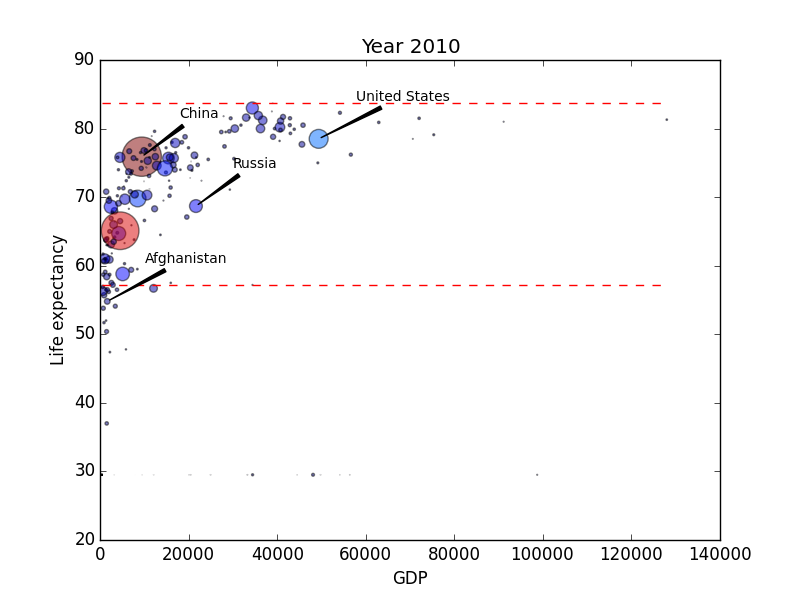
\includegraphics[width=\textwidth]{img/scatter_2010.png}
\end{center}
\end{ex}

\begin{infobox}{Supplementary Files}
The \texttt{country\_data.py} file is available on canvas.
\end{infobox}

\section{The CSV Module}
CSV files are used to store tabular data. They have comma separated values on
each line. Most spreadhseet programs support CSV output and input. Python comes
with the CSV module for reading and writing such files. It supports any
delimiter so you can also manage space-separated and tab-separated data. To
use the module, create a CSV reader using the filename of the data file. For
example, suppose we have the file \texttt{short.csv}. It has column labels
on the first row and columns are separated by commas.

\begin{verbatimcode}
Entity,x         ,y,  z
Fruit tree,1,2,3
Bats, 1, 3, 10
\end{verbatimcode}

We can use the \pythoninline{csv.DictReader} function to parse this data.
It takes an open file as the first argument and returns something that you
can use a for-loop to traverse. It essentially returns a list of dictionaries.
For example,

\begin{pyconcode}
>>> import csv
>>> with open('short.csv') as f:
...     l = [e for e in csv.DictReader(f)]
>>> print(l)
[{'Entity': 'Fruit tree', 'x': '1', 'y': '2', 'z': '3'},
 {'Entity': 'Bats', 'x': ' 1', 'y': ' 3', 'z': ' 10'}]
\end{pyconcode}

Read the documentation to learn about writing CSV files and the
\pythoninline{csv.Sniffer}, which can be used to deduce the format of
a CSV file.

\begin{center}
\url{https://docs.python.org/3/library/csv.html}
\end{center}

\section{Extra Credit Exercise}
\begin{extraex}[parsecsv.py]
The data in the \texttt{plotcountries.py} exercise is from
\url{http://www.gapminder.org/data/}. It was converted to CSV and
parsed using Python's CSV module. See the extra credit if you are
interested in this.  Parse these three CSV files using the CSV module.

\begin{itemize}
\item ``\texttt{indicator gapminder gdp\_per\_capita\_ppp.csv}''
\item ``\texttt{indicator gapminder population.csv}''
\item ``\texttt{indicator life\_expectancy\_at\_birth.csv}''
\end{itemize}

Your data should be the same as the \pythoninline{data} variable in
the \texttt{country\_data.py} file. You may need to pass a keyword
argument in order to open the CSV files: \pythoninline{open(fname,
encoding='utf-8')}.
\end{extraex}

\begin{infobox}{Supplementary Files}
The following files are available on canvas:
``\texttt{indicator gapminder gdp\_per\_capita\_ppp.csv}'',
``\texttt{indicator gapminder population.csv}'',
and ``\texttt{indicator life\_expectancy\_at\_birth.csv}''.
\end{infobox}


\newpage
\section{Submitting}

You should submit your code as a tarball. It should contain all files
used in the exercises for this lab. The submitted file should be named
\begin{center}
  \texttt{cse107\_firstname\_lastname\_lab9.tar.gz}
\end{center}

\begin{center}
  \textbf{Upload your tarball to Canvas.}
\end{center}

\listofexercises
\listofextraexercises

\end{document}


